\documentclass[11pt]{article}

\usepackage[latin1]{inputenc}
\usepackage[T1]{fontenc}      
\usepackage{amsthm}
\usepackage{amssymb}
\usepackage{amsmath}
\usepackage{mathrsfs}
\usepackage{epstopdf}
\usepackage{underscore}
\usepackage{fancyhdr}
\usepackage{hyperref}
\usepackage{graphicx}
\usepackage{hyperref}
\pagestyle{fancy}
\usepackage{geometry}
\geometry{top=2cm, bottom=2cm}
\DeclareMathOperator{\e}{e}

\date{}

\begin{document}
%\maketitle
%\section{}
%\subsection{}

\fancyhf{}
\chead{Network project}
\cfoot{\today}
\rfoot{\thepage/8}
\renewcommand{\footrulewidth}{1pt}
\thispagestyle{empty}

\begin{center}
	{\Large Cyber defense 2\\~\\
	ENSIBS Vannes\\~\\
	2015-2016}
\end{center}
\vspace{3cm}

\begin{center}
	{\huge \textbf{ Report }}
	{\huge \\~\\~ SIP : Communications interception and encryption}
	{\huge
	 \\~\\ \textit{Network basis}}
	\vspace{2cm}
	\begin{figure}[h]

   \centering 
\includegraphics[scale=0.5]{images/EnsibsLogo.jpg}
\end{figure}
\end{center}
\vspace{2cm}

\begin{center}
   {\Large By : 
   Valentin ALLAIRE,
   Dylan COIC,
   Guillaume COUCHARD,
   K�vin FAUVE
	\\~\\ \LARGE Teacher : Ma�l Auzias}
\end{center}

\newpage

\section{Project objectives}

\paragraph{} The objectives of this project are the following : \newline
\begin{itemize}
	\item Set up 2 asterisks servers
	\item Set up 2 soft-phones on our computers or android phones.
	\item Intercept the SIP communication between a soft-phone and the asterisk server.
	\item Intercept the RTP data communication between the 2 soft-phones.
	\item Encrypt the SIP communication using SSL/TLS.
	\item Encrypt the RTP data communication using ZRTP.
	\item Intercept the communication while it's encrypted and prove that the encryption is efficient and reliable.
	\item Doing a trunk SIP between the two asterisks servers.
	\item Try the same things when the two clients are connected on two different asterisks servers.
\end{itemize}
\paragraph{} The difference with the overview is that there is a new objective which is doing a voice recognition on top of the interception of the RTP data communication. \newline

\section{ Why did we not meet all of our objectives ? }

\paragraph{} Mainly because of the lack of time we had and also because when we did the overview we didn't realize it will be a problem to do the encryption. We didn't even try to bypass the SSL/TLS encryption because it takes a lot of time but we think it is possible if the the version of this is SSL v3 for example so we can use the poodle vulnerability. It took us also much time to do the voice recognition because we didn't know the tools and we are not telecoms experts, although it was really cool to learn about it.
We didn't meet the VPN objective also because of the lack of time but we think it can be easily done if we use openVPN for example.
\newline

\section{What we wanted to learn and what we actually learned}

\paragraph{} We wanted to learn more about the VoIP, especially the SIP protocol and we did learn more about that because now we know for example that the SIP is a signaling protocol and RTP is for the data communication between the two soft-phones.
After that we wanted to learn more about the encryption protocols and how it works. We used SSL/TLS for the SIP encryption so we learned a lot about this type of encryption and the certificates. We also learned how to make our own self-signed certificates thanks to this project.
Now we know that to encrypt RTP, we use the SRTP protocol which uses AES 128 bits and SDES to exchange the keys and ZRTP is AES 128 bits too but is using Diffie-Hellman algorithm. 
We also learned what we wanted to learn which was how to configure an asterisk server, intercept a SIP communication and RTP communication and encrypt these communications.
We learned how to do two asterisks server and make them communicate (which is a trunk SIP).
Finally we didn't plan that but we learned how to do a voice recognition using signals analysis.
What we didn't learn because we didn't have the time for it is how to settle a VPN tunnel between the 2 asterisks servers.

\subsection{Challenges encountered}
\paragraph{} During our project we encountered some difficulties, the first one was how to intercept a SIP communication.Indeed, at the beginning we didn't know much about this protocol so we though SIP and RTP were the same thing .... So after we studied the protocol we were able to make the difference and then set up the right filters in Wireshark.
Although that wasn't enough, we connected the two soft-phones, asterisk server and the attacker on the same network and the attacker couldn't intercept all the traffic which was a real problem. Then we understood that we needed to set up the network card into monitor mode and do some arp poisoning (we will explain that in details later on) and that solved the problem. \newline
\paragraph{}The next challenge was to encrypt the SIP communication because at the beginning we didn't really understand how SSL/TLS works. Also, after we understood that, we had to install the right soft-phones because some of them don't handle the SSL/TLS encryption.
Once everything has been done, we had to configure the asterisk server and generate all the certificates, which was hard to do but with a lot of tutorials we managed to succeed.
Finally, the big challenge was to do the voice recognition. \newline


\section{How did we share the code}

\paragraph{} We shared the code using GitHub and e-mails sometimes, for the proof here is the GitHub link : \url{https://github.com/KevinF49/ProjetReseau}
\newpage

\section{Communications Analysis : Wireshark to the rescue !}

\paragraph{}In this section we will mainly talk about the different communications that we did and explain them to you with the help of some Wireshark captures.

\subsection{ARP Communications}

\paragraph{} As the title says, we will show you a capture of some ARP communications in here. We are doing this because this is our way to explain how the attack works and how we tested the security flaw.

\begin{figure}[h]
	\centering 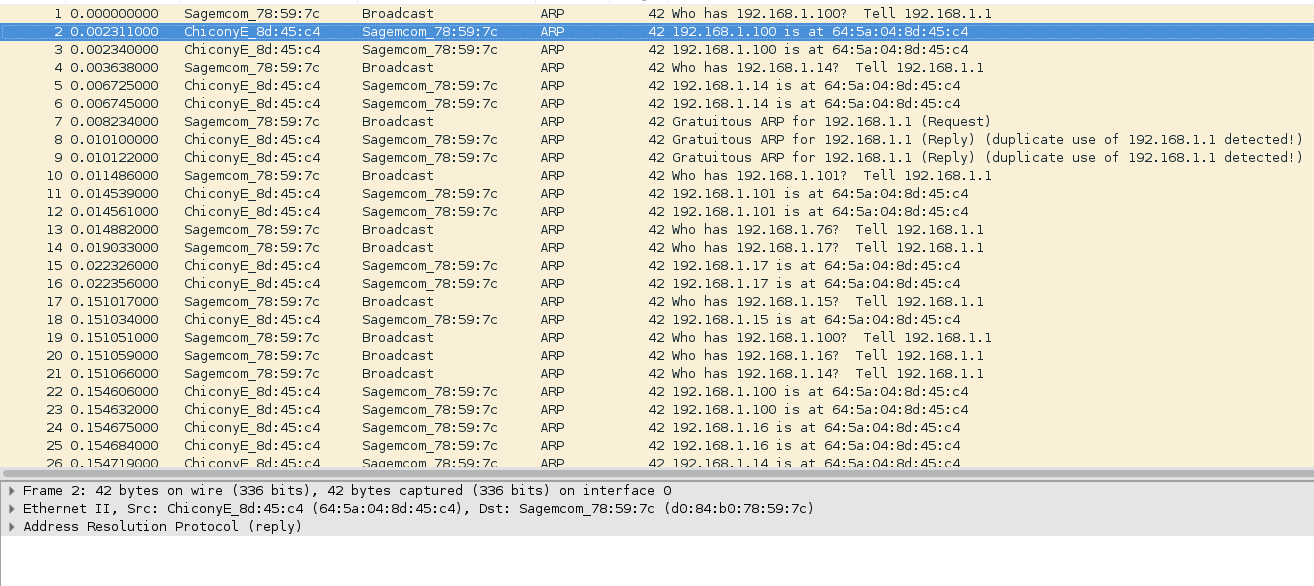
\includegraphics[scale=0.5]{images/arp.png}
	\caption{ARP Flow}
\end{figure}

\paragraph{} First of all, a scan host is established with Ettercap.Then the malicious person sends in broadcast some arp packets and matches his mac address with the ip address of the gateway.
The router sends arp requests to fill his arp table. Thus attacker's mac address answers to all the requests which means his mac address is matched with every IP address on the network.
Thereby, he fills his arp table and all request above the layer 2 are intercepted by him.
The router notices there are two gateways and inform all the devices on the network by sending in broadcast some gratuitous arp packets.
\textit{ChiconyE_8d:45:c4 (64:5a:04:8d:45:c4)} is the attackers' mac address and it is spoofing every IP address on the network.
There is a solution to counter/avoid that "arp poisoning" attack which is setting the arp table in static mode. \newpage


\subsection{SIP Communications}

\paragraph{} In this section we will talk about the results of our project but not how we did it. In order to do that we will show you some Wireshark captures and explain them.

\begin{figure}[h]
	\centering 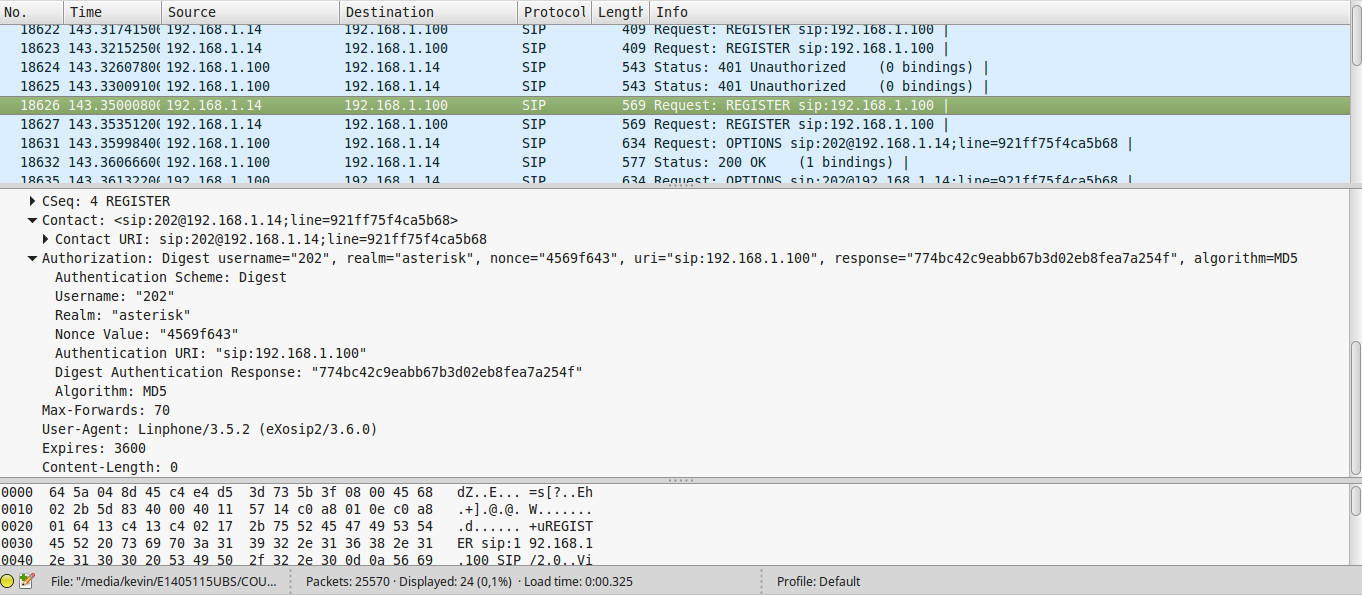
\includegraphics[scale=0.5]{images/REGISTER.jpeg}
	\caption{SIP REGISTER}
\end{figure}


\paragraph{} On this screenshot we can see a weakness of the SIP protocol. User password is hashed 	with MD5 algorithm therefore it's easy to decrypt it. \newline
With this picture only, we have all the information that we need to connect to the asterisk server: \newline
\begin{itemize}
 \item Username \newline
 \item URI \newline
 \item MD5 hash \newpage
\end{itemize}
\subsection{TLS Encryption}

\paragraph{}Now that we saw that SIP is a vulnerable protocol, we will show you that it can be secured if we use SSL/TLS Encryption. For that we used the Blink soft-phone and we created certificates and private/public keys with the openSSL command. 

\begin{figure}[h]

   \centering 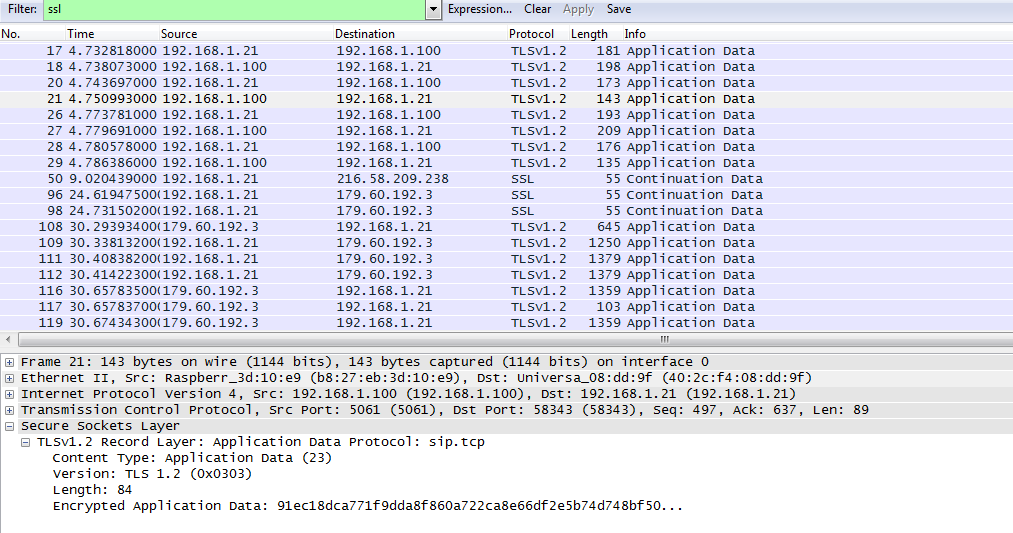
\includegraphics[scale=0.5]{images/TLSSucceed.png}
	 \caption{TLS REGISTER SUCCEED}

\end{figure}

\paragraph{} In this capture you can see that all the packets are encrypted with the TLS Encryption. Just for the record, this is a capture when the user authenticates, which means you could see the right password with SIP but now you just can't see anything because it is encrypted.
\paragraph{}Although, this is only the signalization in this conversation, which means we can still intercept the data packets between the two users, carried by the RTP protocol. \newpage

\subsection{RTP Communications}

\paragraph{} Like we said in the last subsection, the RTP protocol is used to transmit data packets in a VoIP communication. Concretely, it means that voice is carried by this protocol. Which is interesting because we wanted to see if we can intercept these packets and then extract the voice to replay the conversation, and we did.

\begin{figure}[h]
	\centering 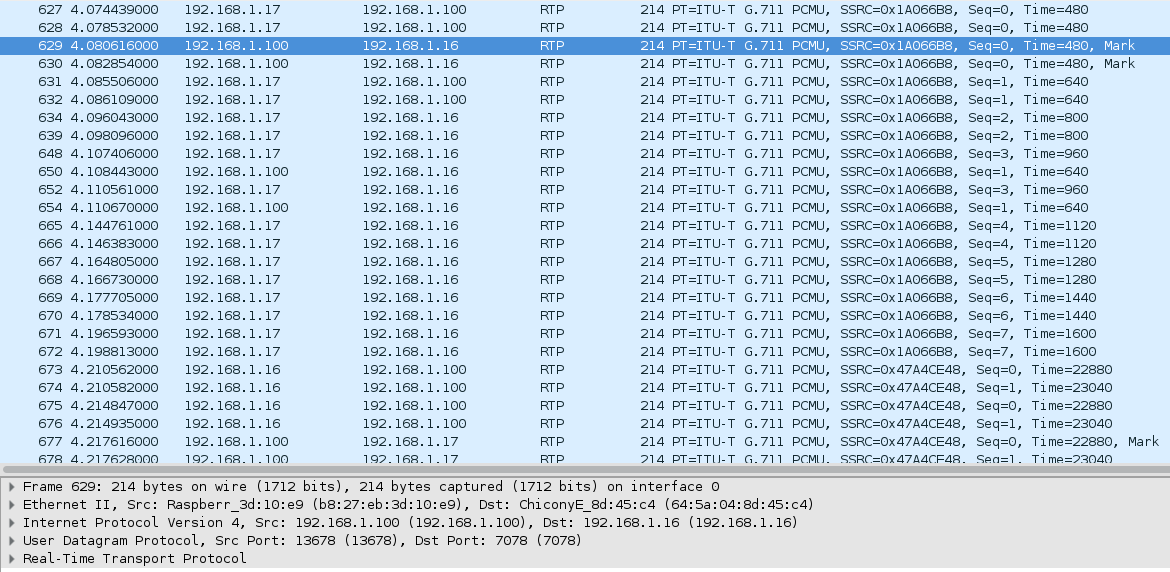
\includegraphics[scale=0.5]{images/rtp.png}
	\caption{RTP}
\end{figure}

\paragraph{} This capture shows the conversation between two soft-phones with the RTP protocol. We can see that the host 192.168.1.17 wants to speak with 192.168.1.16.
But when the host believes that he is sending the packets at the asterisk server, he actually sends the packets to the pirate. That's the same when the real host answers, the packets are for the attacker. 
To sum up, communications are intercepted by the malicious person. This is a hyperlink to a conversation that we intercepted : \href{run:sounds/ConversationGoodQuality.wav}{click to play the sound!}

\newpage

\subsection{SRTP Communications}

\paragraph{} We saw before that RTP is a weak protocol because it is not encrypted, so now we will encrypt it. For that we used SRTP or ZRTP protocols, both are extensions to RTP that incorporates enhanced security features. SRTP for example encrypts RTP using AES 128 bits.

\begin{figure}[h]
	\centering 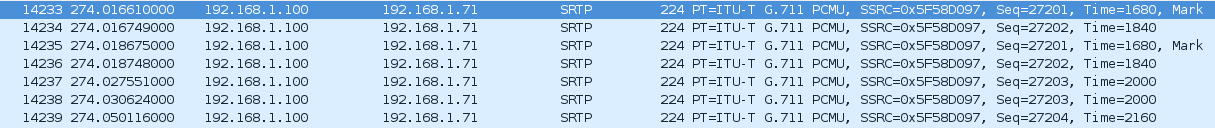
\includegraphics[scale=0.5]{images/srtp.png}
	\caption{SRTP Flow}
\end{figure}

\paragraph{}In this capture the principle is the same that the one above but in this one the conversation is encrypted with SRTP protocol. We won't detail how it works here because this isn't the purpose of this report but basically, it counters our attack because even if we intercept all the SRTP packets, and then we replay the conversation, we will only hear noise because of the encryption, so it's impossible here to hear the voices of the people in a conversation as you can see in this \href{run:sounds/encryptedcom.wav}{audio file} \newline
\newline

\begin{center}
	{\Large \textbf {Conclusion}}
\end{center}

\paragraph{} As you saw when you read this report, it is not about how we configured the servers and soft-phones to get them communicate using VoIP but more about how they do it. For that we had to analyze some Wireshark captures and that is what we explained in here.
To end this report, we would say that SIP along with RTP are really vulnerable therefore if someone wants to set up a ToIP infrastructure they have to secure these protocols using at least SSL/TLS and ZRTP/STRP. Indeed, not only they are vulnerable but the attack is quite easy to do considering it's a simple man in the middle.
We didn't do the best secure network because on top of what we did a VPN can be settled between the two asterisk servers and after that we think it is pretty secure.
\end{document}